\documentclass{pset}
\usepackage{3110}
\usepackage{tikz}

\psnum{4}
\psdue{Thursday, October 17}
\versionnumber{7}

\begin{document}
\maketitle

\standardinstructions

\medskip
\hrule
\hrule
\section*{Getting started}
This problem set is long; we recommend you start thinking about all of the
parts early.  Parts two and three depend on part one, but you only need to
implement one of the modules (\code{Floats}) in part one to get started on them.
The things you have to do are indicated by ``Exercise'' in the writeup, and
are labeled ``TODO'' in the release code.

The GUI for this problem set requires some additional OCaml libraries; the file
\filename{README.txt} in the release contains instructions for compiling and
running the project.

\pagebreak
\section*{Introduction}
In many applications, users want to rearrange a collection of geometric shapes
while keeping them from overlapping with each other.  For example, users like
to rearrange windows on their desktops while keeping each window entirely
visible.  Without an automated way to keep them from overlapping, users must
carefully adjust the boundaries of the windows if they want to avoid large gaps
between the windows.  The same user interface feature is useful in other
applications, such as computer aided design, graphics applications, and games.

In this assignment, you will be building a library that allows users to drag and
drop shapes while keeping them from intersecting each other.  You will use the
library to build a simple
``\link{http://en.wikipedia.org/wiki/Tangram}{tangrams}'' game.

The correctness of geometric algorithms depends on the properties of the numbers
used to represent the coordinates of the shapes.  You will implement a variety
of number types to investigate the tradeoffs of various representations.

Finally, this assignment contains a small problem related to mutability.

\part{Numbers}

For this portion of the assignment, you will implement a variety of modules,
each defining a representation of a set of numbers and the operations available
for those numbers.

Your number modules will each implement one of the following interfaces (we have
provided these signatures in \filename{numbers.ml}):
\begin{itemize}
\item A \link{http://www.proofwiki.org/wiki/Definition:Quotient_Set}{\code{Quotient}}
      represents a set of elements, which we will refer to as
      \code{number}s.  The only operation provided by \code{Quotient} is the
      \code{(===)} function, which defines the notion of equality for the set of
      \code{number}s.

\item Just as \code{Quotient} defines a notion of equality
      between numbers, \link{http://en.wikipedia.org/wiki/Abelian_group}{\code{Group}}
      defines a notion of addition.  In addition to the \code{(+)} operation,
      \code{Group} requires a number called \code{zero}, and for each number
      $x$, an additive inverse \code{-$x$}.  Note that OCaml writes the
      negation operation as \code{(~-)}.  That is, \code{(~-) x} is the same as
      \code{-x}.

\item \link{http://en.wikipedia.org/wiki/Commutative_ring}{\code{Ring}} extends \code{Group} by adding a notion of
      multiplication.  It also requires a multiplicative identity called
      \code{one}.

\item A \link{http://en.wikipedia.org/wiki/Field_\%28mathematics\%29}{\code{Field}}
      is a ring where every number $x$ has a
      multiplicative inverse $x^{-1}$.  This allows us to define
      division: $x/y$ is just $xy^{-1}$.
      
\item \link{http://en.wikipedia.org/wiki/Ordered_ring}{\code{OrderedRing}} and
      \link{http://en.wikipedia.org/wiki/Ordered_field}{\code{OrderedField}}
      add a notion of ordering to
      rings and fields respectively.  We only require implementors to provide
      a function that determines if a number is negative, but
      comparison operations like \code{(<)} and \code{(>)} can
      be defined in terms of \code{is_non_neg} (you will do this in exercise 2
      below).

\item \code{NiceRing} and \code{NiceField} require additional useful functions:
      the ability to convert a \code{number} to an OCaml \code{float}, and a
      function for printing a \code{number} onto the console.  You can register
      these formatting functions with the OCaml toplevel using the
      \code{#install_printer} command; this will cause the toplevel to use that
      function to print out values of your number type.  See the
      toplevel documentation and the documentation for the OCaml \code{Format}
      module for more details.
\end{itemize}

These concepts (with the exception of \code{NiceRing} and \code{NiceField}) are
borrowed from the field of abstract algebra\footnote{note that our groups are
technically Abelian groups, and our rings are technically commutative rings
with identity}.  In the same way that modular programming allows us to apply
single functions to a large number of data types, these modular definitions
have allowed algebraists to prove single theorems that apply to a large number
of mathematical structures.

In order for the operations defined by these concepts to make sense, they must
obey certain properties (axioms).  For reference, we have provided modules that
encode these properties as functions.  For example, the multiplication
operation only makes sense if it is commutative, associative, distributes over
addition, and if one is a multiplicative identity.  These properties are tested
(for individual numbers) by the \code{times_commutative},
\code{times_associative}, \code{times_distributive} and \code{times_identity}
functions.  A module \code{R} that implements \code{Ring} is only valid if for
all inputs $a$, $b$, and $c$, each of the functions of the \code{RingProperties (R)} module return true.  Similarly, the other \code{Properties} modules
(\code{QuotientProperties}, \code{GroupProperties}, \code{FieldProperties}, and
so on) encode the properties of the other module types.

\exercise{Simple number types}
Implement the following modules and functors in \filename{numbers.ml} (you may
want to implement some of these in terms of others):
\begin{itemize}
\item \code{module Ints : NiceRing}, using \code{int} as the number type.
\item \code{module Integers : NiceRing}, using large integers as the number type.
      You may either use your implementation of big integers from problem set 2,
      or OCaml's built-in \code{Big_int} module.
\item \code{module Floats : NiceField}, using \code{float} as the number type.
      Because floating point arithmetic is inexact, you should consider two
      \code{float}s to be equal if they differ by less than $10^{-6}$.
      \begin{note}{Warning}This should be your only number module that uses the \code{float} type (with the exception of the \code{float_of_number} functions).\end{note}
\item \code{module Root23 : NiceRing} that contains numbers of the form
      $a + b\sqrt{2} + c\sqrt{3} + d\sqrt{6}$ where $a$,$b$,$c$ and $d$ are
      integers.  In addition to the \code{NiceRing} functions, this module
      should expose the \code{number}s \code{sqrt2}, \code{sqrt3}
      and \code{sqrt6} representing $\sqrt{2}$, $\sqrt{3}$ and $\sqrt{6}$
      respectively.
      \begin{note}{Hint 1} $a_1 + a_2\sqrt{2} + a_3\sqrt{3} + a_6\sqrt{6}$ is
      zero if and only if $a_1$, $a_2$, $a_3$ and $a_6$ are zero.  This fact may
      help you with \code{Root23.(===)}.
      \end{note}
      \begin{note}{Hint 2} For \code{Root23.is_non_neg}, try working out the
      solution for numbers of the form $a + b\sqrt{2}$ first, and then writing
      numbers in the form $(a + b\sqrt{2}) + (c + d\sqrt{2})\sqrt{3}$.
      \end{note}
\item \code{module FieldOfFractions (R : NiceRing) : NiceField} should
      represent numbers as fractions of \code{R.number}s.  You are not required
      to store the fractions in lowest terms.
\item \code{module Rationals : NiceField} should implement the rational numbers.
      You are not required to store the fractions in lowest terms.
\item \code{module Rot15 : NiceField} should contain the rationals as well as
      the numbers $\cos 45^\circ$, $\sin 45^\circ$, $\cos 30^\circ$, and
      $\sin 30^\circ$.
\begin{note}{Hint}these can all be expressed in terms of $\sqrt{2}$ and $\sqrt{3}$.\end{note}
\end{itemize}

You may find the \code{include} and \code{open} statements useful for this
problem (and throughout the remainder of the problem set).

\exercise{Implement utility functors}
In our definitions of \code{Quotient}, \code{Group}, \code{Ring} and so on, we
provided a minimal set of functions; this makes it easier to implement
these interfaces.  For example, a module that implements \code{OrderedRing}
only needs to provide the \code{is_non_neg} function; but when using numbers
from ordered fields, it is useful to have ordering functions such as \code{(>)},
\code{(<)}, \code{(>=)}, and \code{(<=)}.

Implement the following utility functors in
\filename{numbers.ml} to provide these useful operations:
\begin{itemize}
\item \code{module QuotientUtils (Q : Quotient)} should define the not-equal
      function \code{(<>)} in terms of the \code{(===)} function on \code{Q}.
\item \code{module GroupUtils (G : Group)} should define the binary \code{(-)}
      function in terms of the group operations on \code{G}.
\item \code{module RingUtils (R : Ring)} should define the \code{number_of_int}
      function\footnote{For those of you who like abstract algebra, the existence
      and properties of this function means that the integers are initial in
      the category of rings}, which converts an integer into an
      \code{R.number}.
\item \code{module FieldUtils (F : Field)} defines the division function for
      \code{F.number}s.
\item \code{module OrderedRingUtils (R : OrderedRing)} provides the comparison
      operations mentioned above (\code{(<)}, \code{(>)}, \code{(<=)} and
      \code{(>=)}, \code{min} and \code{max}).  It should also adapt the
      ordered ring interface to the standard \code{Set.OrderedType} interface,
      so that elements of an ordered ring can be used in OCaml \code{Set}s and
      \code{Map}s.
\item \code{module OrderedFieldUtils (F : OrderedField)} should simply combine
      the operations from \code{OrderedRingUtils} and \code{FieldUtils}.
\end{itemize}

Once you have defined these modules, you can work with the numbers in a given
group, ring or field very easily:
\newcommand{\sq}{\sqrt{\rule{0em}{.5em}}}
\begin{ocaml}
    # module R  = Numbers.Root23;;
    # module RU = Numbers.OrderedRingUtils (R);;
    # open R;;
    # open RU;;
    # #install_printer format;;

    # zero;;
    - : R.number = 0

    # one;;
    - : R.number = 1

    # one + sqrt2;;
    - : R.number = 1+$\sq$2

    # (one + sqrt2) * (one - sqrt3) + one + sqrt2 - sqrt6;;
    - : R.number = 2+2$\sq$2-$\sq$3-2$\sq$6

    # let x = one + sqrt2;;
    val x : R.number = 1+$\sq$2

    # let y = (number_of_int 7) - sqrt6;;
    val y : R.number = 7-$\sq$6

    # x * y;;
    - : R.number = 7+7$\sq$2-2$\sq$3-$\sq$6
\end{ocaml}

\begin{note}{Note}
The way that the toplevel displays your output will depend on your
implementation of \code{Root23.format}.  This function is intended for your own
benefit while debugging; you are free to format your numbers any way you
choose.
\end{note}

\exercise{Implement real numbers}
Implement arbitrary precision real numbers in
\filename{numbers.ml}.  Your implementation should implement the
\code{NiceField} interface.

You should provide a function \code{approximate} which given an integer $k$,
and a real number $x$, produces a rational number that is within $10^{-k}$ of
$x$.  That is,
\begin{displaymath}
\left|\code{x} - (\code{approximate x k})\right| < 10^{-\code{k}}
\end{displaymath}
In addition, you should provide a function \code{create} that accepts a
function \code{f} such that the sequence \code{f 0}, \code{f 1}, \code{f 2},
$\dots$
converges to a real number $x$; \code{create f} should
return $x$.  The input to create is assumed to converge at a rate of $10^{-k}$;
the behavior of \code{create} is undefined for sequences that do not converge.

Your implementations of \code{(===)} and \code{is_non_neg} are not required to
terminate, but they should terminate when possible.

\begin{note}{Hint}
If you get stuck while trying to come up with a representation for
\code{Real.number}, think carefully about the types and specifications of
\code{create} and \code{approximate}.  If you can implement these functions
well, the rest of the \code{NiceField} operations will follow.
\end{note}

To give you some interesting real numbers to play with, you should provide an
exact representation of the numbers $\pi$ and $e$.  There are many techniques
for doing so; one possibility is to use the Taylor series expansions for the
arctangent and exponential functions respectively.

\part{Geometry}

In this portion of the assignment, you will build on the number types you
defined in part one to construct a collision-avoiding drag-and-drop library for
convex polygons in the plane.

\begin{note}{Note}
This portion of the assignment depends on part 1, but you do not need to
implement all of part 1 to get started on part 2.  We recommend that you
implement \code{Numbers.Floats} first, and use it to get started on this
portion.
\end{note}

Suppose a user clicks on a shape $S$ and drags it from a point $x$ to a point
$y$ (see Figure~\ref{fig:drag}.  Suppose further that we wish to prevent $S$
from overlapping with any of the obstacles $O_1$, $O_2$, \dots, $O_n$.  If
placing $S$ at $y$ does not cause it to intersect the obstacles, then it would
make sense to simply place $S$ at $y$.  However, if placing $S$ at $y$ would
cause an intersection, what should we do?

One approach is to place $S$ at the closest point to $y$ that doesn't cause any
overlaps.  It turns out that this specification provides a very natural drag
and drop experience, because it allows the user to easily adjust the position
of adjacent objects.  This scheme is illustrated in Figure~\ref{fig:drag}.

We can compute these points as follows.  When the user clicks on a shape, we
compute a representation of the set of points $y$ such that if $S$ were placed
at $y$, there would be an overlap.  If $O = O_1 \cup O_2 \cup \cdots \cup
O_n$, then this set consists of the points $\{p - q \mid p \in O, q \in S\}$.
This is known as the
\link{http://en.wikipedia.org/wiki/Minkowski_addition}{Minkowski difference} of
$O$ and $S$; it is often written $O \ominus S$.  It is the shaded area in
Figure~\ref{fig:drag}.

Whenever the user moves the mouse to a new location $y$, we can use this
representation to determine whether $y \in O \ominus S$, and if it is, we can
find the closest point to $y$ on the boundary of $O \ominus S$.  We can then
place $S$ at this point.

For this project, we will assume that the shape to be dragged and the obstacles
are all convex polygons, represented as lists of points.  Points will be
represented as pairs of \code{number}s from a given \code{Numbers.OrderedField}.
This means that your geometry code must be included in a functor parameterized
on an \code{OrderedField}.

\exercise{Implement Minkowski difference for convex polygons}
In the file \filename{geometry.ml}, write a function
\code{minkowski_difference_convex} that computes the Minkowski difference of
two convex polygons represented as \code{point list}s.

Computing the Minkowski difference of convex polygons is a straightforward
process, because it is simply the convex hull of the differences of all pairs
of polygon corners from each of the two input polygons.  See
Figure~\ref{fig:mink} for an illustration.

We leave it up to you to find and implement an algorithm for computing the
convex hull.  We encourage you to use the internet to find an algorithm, and
you may even look at open source implementations if you wish, but you must
write your code yourself.

\exercise{Implement Minkowski difference}
The next step is to compute the Minkowski difference of the dragged shape with
the entire set of obstacles.  This can be accomplished by computing the
Minkowski difference of the dragged shape with each obstacle, and the taking
the union of the resulting differences.

Computing the union of many polygons is a difficult problem, because the union
of two polygons may contain holes, and even degenerate zero or one dimensional
holes.  These holes are quite important for drag and drop, because they
represent spaces between the obstacles where one may want to place the dragged
shape.

In the \code{Region} module we have provided you with an implementation of
polygon union.  Use this module to write a function \code{minkowski_difference}
that computes the Minkowski difference of a list of obstacles (represented as
\code{point list}s) with the dragged shape.  This function should return a
\code{Region.region}.

\begin{figure}
\begin{center}
\begin{tikzpicture}
\fill[BackgroundGreen] (4.7,2.25) -- (6.75,2.25) arc (180:135:.75)
                       -- ++ (1,1) arc (135:45:.75)
                       -- ++(1,-1) arc (45:-90:.75)
                       -| (8.45,-.5) arc (0:-90:.75)
                     -- ++(-3,0) arc (-90:-180:.75)
                     -- ++(0, 2) arc (180:90:.75);

\draw[fill=NoteBackground] (5,-1) -- (8,-1) -- (8,1) -- (5,1) -- cycle;
\node[anchor=south] at (6.5,-1) {$O_1$};

\draw[fill=NoteBackground] (7.5,1.75) -- (9.5,1.75) -- (8.5,2.75) -- cycle;
\node[anchor=south] at (8.5,1.75) {$O_2$};

\foreach \p in {
  (0,0), (1.8,.5), (3.8,1), (5.8, 1.75),
  (6.55, 1.75), (8.75,-.25), (8.75,-.5), (9, -1), (11, -1)
} {
	\draw[fill=white] \p circle (.75);
	\draw \p + (-0.3,0.5) circle (2pt);
}

\draw[thick,blue] plot[smooth,tension=1,mark=*] coordinates {
  (-0.3,0.5) (1.5, 1) (3.5, 1.5) (5.5, 1.25) (6.25, 0.5) (7, 0.25) (7.7, 0) (8.7, -.5) (10.7, -.5)
};

\node[below right] at (-0.3,0.5) {$x$};
\node[below right] at (10.7,-.5) {$y$};
\node[below] at (0,-.75) {$S$};


\draw[dotted] (5.5,1.25) -- (5.5,2.25);
\draw[dotted] (6.25,0.5) -- (6.25,2.25);
\draw[dotted] (7,0.25)   -- (8.3,0.25);
\draw[dotted] (7.7,0)    -- (8.3,0);

\draw[dashed] (4.7,2.25) -- (6.75,2.25) arc (180:135:.75)
		       -- ++ (1,1) arc (135:45:.75)
		       -- ++(1,-1) arc (45:-90:.75)
		       -| (8.45,-.5) arc (0:-90:.75)
		       -- ++(-3,0) arc (-90:-180:.75)
		       -- ++(0, 2) arc (180:90:.75);


\end{tikzpicture}
\end{center}
\caption{The positions that the circle $S$ takes as it is dragged along the
blue path.  The yellow shapes $O_1$ and $O_2$ are the obstacles.  The shaded
area contains all points $y$ such that placing $S$ at $y$ would cause $S$ to
intersect one of the obstacles.  At each point, the circle is placed at the
closest point to the mouse location that is not in this set.  The circle is only
for illustration; you will only be handling polygons.}
\label{fig:drag}
\end{figure}

\begin{figure}
\begin{center}
\begin{tikzpicture}
\newcommand{\apts}{0/0/1/left, 2/2/2/right, 2/4/3/right, 0/2/4/left}
\newcommand{\bpts}{0/0/1/left, 1/0/2/right, 0.5/1/3/above}

\draw (0,2) \foreach \x / \y / \n / \side in \apts {
            -- (\x,\y) node[fill,circle,scale=0.3] {} node[\side] {$a_\n$}
};

\begin{scope}[xshift=1cm,yshift=2cm]
\draw[xshift=4cm] (0.5,1) \foreach \x / \y / \n / \side in \bpts {
                        -- (\x,\y) node[fill,circle,scale=0.3] {} node[\side] {$b_\n$}
};
\end{scope}

\begin{scope}[xshift=10cm,yshift=1cm]

\draw (-1,0) -- (-1,2) -- (1,4) -- (2,4) -- (2,2) -- (1.5,1) -- (-.5,-1) -- cycle;

\foreach \ax / \ay / \an / \aside in \apts
  \foreach \bx / \by / \bn / \bside in \bpts
    \fill (\ax-\bx,\ay-\by) node[fill=white, below] {$x_{\an\bn}$} node[fill,circle,scale=0.3] {};
\end{scope}

\end{tikzpicture}
\end{center}
\caption{The Minkowski difference of convex polygons can be computed by finding
the convex hull of the differences of all pairs of points.  In the diagram,
$x_{ij} = a_i - b_j$.}
\label{fig:mink}
\end{figure}

\part{Tangrams}

In the last portion of the assignment, you will integrate your geometry code
into the tangrams application.

The logic of the game is very simple; users get a handful of simple shapes
which they are supposed to arrange into a single large shape.  The shapes are
shown in Figure~\ref{fig:sshot}; in fact this is a screenshot of what you will
see as soon as you implement a \code{NiceField} and run the user interface.

\begin{figure}
\begin{center}
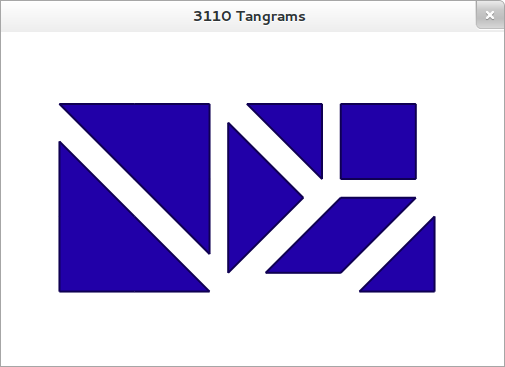
\includegraphics[height=3in]{sshot.png}
\end{center}
\caption{The tangrams user interface}
\label{fig:sshot}
\end{figure}

\exercise{Implement drag and drop}

Your goal is to implement the drag and drop behavior for the application in
\filename{game.ml}.  The UI code will call the \code{click}, \code{move_to} and
\code{unclick} functions whenever the user performs the corresponding actions.
It will then call the \code{obstacles} and \code{selection} functions to
determine what to draw on the screen.

The \code{obstacles} function should return the list of undragged polygons,
while \code{selection} should return the polygon that is currently being
dragged (or \code{None} if the user is not currently dragging).  You are also
free to return extra points or lines to draw using the \code{extra_points} or
\code{extra_lines} functions; these will be drawn by the UI and may aid you in
debugging.

As described above, when the user clicks, you should compute the Minkowski
difference of the polygon they clicked on with all of the other polygons.  When
they drag the mouse to a point $p$, you should find the closest point to $p$
that is not in that difference (you should use \code{Region.find_closest} for
this).

The code that actually constructs and runs the UI is contained in
\filename{main.ml}.  If you wish to test your code with a different number type
you should modify that file to load the appropriate module.  You can then build
and run the application as described in \filename{README.txt} in the release
file.

\part{Written questions}

\exercise{Written questions}
Answer these questions in the file \filename{written.txt} or
\filename{written.pdf}.  Don't forget that most of the \code{Properties}
modules include other \code{Properties} modules.  For example,
\code{FieldProperties} contains \code{plus_commutative} as well as
\code{times_commutative}, because the \code{FieldProperties} extend the
\code{GroupProperties}.


\begin{enumerate}[(a)]
\item We asked you to implement the \code{Ring} interface for the \code{Ints}
      and \code{Integers}, but integers also have a built-in division operator
      \code{(/)}.  If we used integer division to implement the \code{Field}
      interface, which of the field properties would be violated?  Give a set of
      inputs to the corresponding \code{FieldProperties} function that
      demonstrate that the property is violated.

\item If you run your tangrams game using \code{FieldOfFractions(Ints).number}s,
      you will see strange behavior.  This is because some of the properties of
      \code{NiceRing} are not satisfied by the \code{Ints}.  Give a set of
      inputs and a function from \code{OrderedRingProperties(Ints)} that demonstrate
      a property that is violated.

\item Your tangrams game will also not work correctly using the \code{Floats},
      although you may have to play with it a bit more to see visible errors.
      Again, these failures can be ascribed to a failure to implement the
      \code{FieldProperties} perfectly.  Give a set of inputs and the
      name of a \code{FieldProperties(Float)} function that demonstrate the
      failure.

\item Your arbitrary precision real numbers are able to implement every real
      number exactly.  Explain in one or two sentences why they are not the
      ideal number implementation for your tangrams game.
\end{enumerate}

\end{document}

